\documentclass[../full_thesis/full_thesis.tex]{subfiles}


% Default image directory
\newcommand{\thisdir}{../rotating_frame}
\graphicspath{{\thisdir/img/}}

\begin{document}
In this section, we will develop intuition about the precession of a biaxial
body under the action of the \citet{Goldreich1970} dipole spin-down torque.  We
will do this by solving the Euler rigid-body equations numerically and
comparing with known analytic solutions and approximate solutions in the
literature. This section considers solution exclusively in the rotating body frame
of the star. In the torque-free case, this means there is only one timescale: the
precession period.  The torque introduces two new timescales; we will consider
how solutions depend on the ordering of these timescales and discuss which of
these are physically relevant to real neutron stars.

\section{Defining the model}
\label{sec: defining the model}

Euler's rigid-body equations describe the motion of a rigid-body in a rotating
reference frame. To derive these, we begin with Euler's second law for the
angular momentum $\mathbf{J}$ in the inertial frame
\begin{equation}
    \frac{d\mathbf{J}}{dt}=\mathbf{T},
\end{equation}
where $\mathbf{T}$ is the applied torque. The angular momentum is the product
of the moment of inertia tensor and the spin-vector, $\mathbf{J}=I \spin$; in the inertial
frame both of these quantities vary in time. We can simplify by
transforming to a frame fixed in the rotating frame of the rigid-body and
aligning the axes with the principal axes of $I$. In such a frame, the moment
of inertia tensor is constant and diagonal. The transformation to a rotating reference
frame requires a modification of the time derivative in Euler's second law, see
\citet{Landau1969} for details. The result is Euler's rigid-body equations in
the rotating frame
\begin{equation}
    \frac{d\mathbf{J}}{dt} + \spin \times \mathbf{J} = \mathbf{T}.
    \label{eqn: eom}
\end{equation}
To begin with, we will restrict ourselves to consider only biaxial bodies with
principal moments given by
\begin{equation}
I_{x} = I_{y} = I_{0} \;\;\;\;\;\;\; I_{z} = I_{0}(1+\epsI).
\end{equation}
For neutron stars, their extreme gravity ensures that $\epsI \ll 1$ such that
we take a typical moment of inertia to be
\begin{equation}
I_{0} = \frac{2}{5}MR^{2} \approx 10^{45}\textrm{g cm}^{2} M_{1.4}R_6^{2},
\end{equation}
where $M_{1.4} = 1.4 M_{\odot}$ and $R_6=10^{6}$~cm are typical values.

In Cartesian coordinates, equation \ref{eqn: eom} gives us three coupled ODEs
for $\omega_{x}, \omega_{y}$ and $\omega_{z}$. In the torque-free case analytic
solutions can be found as we demonstrated in section \ref{sec: free precession}.

Neutron stars are acted on by torques from both their electromagnetic (EM)
dipole and, if $\epsI \ne 0$, they may also be acted on by torques from the
emission of gravitational waves. For now we will consider only the former
effect which dominates for isolated neutron stars observed as pulsars. To model
this EM torque, we imagine a dipole $\m$ frozen into the star. In the rotating
frame, the body is axially symmetric about the $\z$ axis; therefore we are free
to fix the dipole in the $\x-\z$ plane at an angle $\chi$ to the $\z$ axis
without loss of generality. \citet{Deutsch1955} demonstrated such a dipole
exerts a torque on the star, which has two components. We present it here in the
form found in \citet{Goldreich1970},
\begin{equation}
\boldsymbol{T}=\frac{2R}{3c} I_{0}\epsA\omega^{2}
               (\spin \times \hat{\boldsymbol{m}})\times \hat{\boldsymbol{m}}
               + \epsA I_{0}(\spin \cdot \hat{\boldsymbol{m}})
               (\spin \times \hat{\boldsymbol{m}}),
\label{eqn: torque}
\end{equation}
where $\epsA$ is an effective magnetic `deformation' as defined by \citet{Glampedakis2010}
and given by 
\begin{align}
\epsA = \frac{m^{2}}{I_{0}R c^{2}},
\end{align}
this can be related to the surface magnetic field strength by
\begin{equation}
    B_{0} = \left(\frac{4 \epsA I_{0} c^{2}}{R^{5}}\right)^{1/2}.
    \label{eqn: magnetic field epsA}
\end{equation}

The first term in the Deutsch torque is often referred to as the
\emph{spin-down}, or \emph{braking} torque. As the name suggests, it is
responsible for the power law retardation of spin frequency and has an
associated timescale $\tau_{S}$. The second term is known as the
\emph{anomalous} torque which acts on a timescale $\tau_{A}$. The three
timescales (including the precession timescale) in this problem are then given
by
\begin{equation}
\tau_{P}=\frac{2\pi}{\epsilon_{I}\omega},  \;\;\;\;\;
\tau_{A}=\frac{2\pi}{\epsA\omega},  \;\;\;\;\;
\tau_{S}=\frac{3c}{2R}\frac{1}{\epsA\omega^{2}}.
\label{eqn: torque timescales}
\end{equation}
The ordering of these timescales characterises the type of solutions found to
Eqn.~\eqref{eqn: eom} with the torque of Eqn.~\eqref{eqn: torque}. There are
six potential orderings, however by considering the ratio $\tau_{A}/\tau_{S}
\sim v/c$, where $v$ is the equatorial velocity, we see that $\tau_{A} \ll
\tau_{S}$ reducing the number of possible orderings to three.

We now have the basic components of a neutron star: a biaxial rigid-body spun
down by a dipole torque. To help familiarise the reader with the notation, in
Table~\ref{tab: definitions} we list the spherical components of spin-vector
and magnetic dipole and also show their projection onto the $\x-\z$ plane in
Fig.~\ref{fig: sketch01}. We work in a system of coordinates where the polar
angle is that made with the $\z$ axis and the azimuthal angle is the angle between
the projection of the vector onto the $\x-\y$ plane and the $\x$ axis.
\begin{table}[ht]
\centering
\begin{tabular}{|l|c|c|c|c|} \hline
 \multicolumn{2}{|c|}{} & Magnitude & Polar angle & Azimuthal angle \\ \hline
Spin vector  & $\boldsymbol{\omega}$ & $\omega$ & $a$ & $\phi$ \\ \hline
Magnetic dipole &  $\boldsymbol{m}$ & $m$ & $\chi$ & 0 \\ \hline
\end{tabular}•
\caption{Table of spherical components for the spin-vector and magnetic dipole}
\label{tab: definitions}
\end{table}

\begin{figure}[ht]
\centering
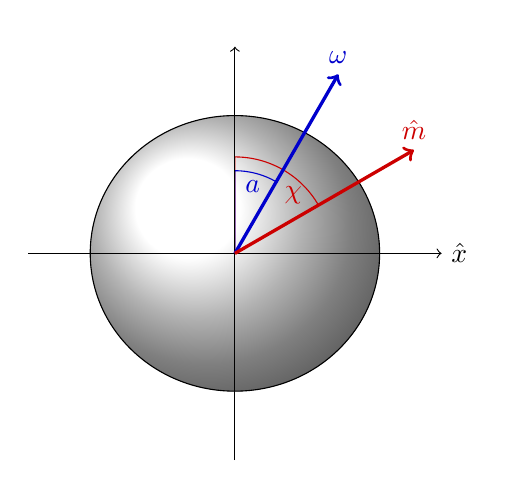
\begin{tikzpicture}[scale=1.75] 
	% Define some things

	\def\costhirty{0.8660256}
	\def \mag{1.5}

	\def\cosbeta{0.984}
	\def\sinbeta{0.173}

	% Colors
	\colorlet{anglecolor}{blue!80!black}
	\colorlet{sincolor}{red}
	\colorlet{tancolor}{orange!80!black}
	\colorlet{coscolor}{blue}

	% Styles
	\tikzstyle{axes}=[]
	\tikzstyle{important line}=[very thick]
	\tikzstyle{information text}=[rounded corners,fill=red!10,inner sep=1ex]

	% Draw the shaded star
	\def\R{1.0} % sphere radius
	\filldraw[ball color=white] (0,0) ellipse (1.05 and 1.0);

	% Draw the angles
	\draw[draw=red!80!black] (0,0) -- (0pt,7mm) arc(90:30:7mm);
	  \draw (45:6mm) node[red!80!black] {$\chi$};


	\draw[draw=blue!80!black] (0,0) -- (0pt,6mm) arc(90:60:6mm);
	  \draw (75:5mm) node[blue!80!black] {$a$};



	%\draw[draw=green!60!black] (0,0) -- (12mm*\costhirty,12mm*0.5) arc(30:60:12mm);
	 % \draw (45:11mm) node[green!60!black] {$\alpha$};



	% Draw the body frame axis
	\draw[->] (-1.5,0) -- (1.5,0) node[right] {$\hat{x}$};
	\draw[->] (0,-1.5) -- (0,1.5) node[above] {$\z$};

%	% Draw the effective body frame axis
%	\draw[draw=black] (0,0) -- (0,13mm) arc(90:100:13mm);
%%	  \draw (95:11mm) node[black] {$\beta$};
%	\draw[draw=magenta] (0,0) -- (-8.1*\sinbeta mm, 8.1*\cosbeta mm) arc(100:60:8.1mm);
%	  \draw (80:9.2mm) node[magenta] {$a'$};
%
%	\draw[dashed,->] (-1.5*\cosbeta,-1.5*\sinbeta) -- (1.5*\cosbeta,1.5*\sinbeta) node[right] {$x'$};
%	\draw[dashed,->] (1.5*\sinbeta,-1.5*\cosbeta) -- (-1.5*\sinbeta,1.5*\cosbeta) node[above] {$z'$};




	% Define omega to have unit magnitude and lie at 30 degrees to the z axis
	{\draw[color=blue!80!black,very thick,->] (0,0,0) -- (\mag*0.5,\mag*\costhirty) node[anchor=south]{$\omega$};}%

	% Define m to have unit magnitude and lie at 60 degrees to the z axis
	{\draw[color=red!80!black,very thick,->] (0,0,0) --(\mag*\costhirty,\mag*0.5) node[anchor=south]{$\hat{m}$};}%

\end{tikzpicture}

\caption{A sketch of the  $\x-\z$ plane,  the magnetic dipole lies solely in
this plane such that its azimuthal component is always zero.  Only the
projection into this plane of the spin-vector is shown, in general it has an
azimuthal component given by $\phi$.}
	\label{fig: sketch01}
\end{figure}•

In the following sections we will develop our intuition for the different types
of solutions to this model. These results are calculated by 
exact numerical evolution of Eqn.~\eqref{eqn: eom} with the torque defined in
Eqn.~\eqref{eqn: torque}. The simulations model a a NS with a magnetic field of
$B_{0}\approx10^{13}$~G and a radius $R=10^{6}$~cm. We must also provide an
initial condition for the angular frequency $\omega$. This is not the spin
frequency at the birth of the NS, but the frequency at the start of the observation;
typical values are of the order $\sim 10$~rad/s. However, at this frequency the
numerical solutions are computationally expensive. To reduce the time required
to produce a solution we will work with an initial frequency of $\omega =
10^{4}$~rad/s. This does not change the form of solution, only the timescales
over which they evolve.

\FloatBarrier
\section{Spherical star}
\label{sec: spherical}

We begin by considering the simplest case: a spherical star with $\epsI=0$
under the influence of the spin-down torque.  This model was first considered
by \citet{Davis1970} and separately by \citet{Michel1970}; both sets of authors
discovered that torque causes the spin axis to align with the magnetic axis on
the spin-down timescale.

To observe this behaviour, we set $\chi=30^{\circ}$ with the spin-vector
initially at $a=50^{\circ}$ and $\epsA=5\times10^{-11}$. Evolving the model
numerically, we plot the spherical components of the spin-vector in figure~\ref{fig:
NS spherical}. This shows a brief spin-down which halts once the spin-vector
aligns with the magnetic dipole $a \rightarrow \chi=30^{\circ}$.  The azimuthal
angle $\phi$ does not vary; this is expected since precession, a monotonic
increase in $\phi$, does not occur for spherical bodies. This result agrees
with the analytic calculations: the alignment occurs on the spin-down time
scale $\sim 3.6\times 10^{8}$~s.
\begin{figure}[ht]
\centering
	\centering
	\includegraphics[width=0.5\textwidth]
     {{Spherical_Plot_no_anom_chi_30.0_epsI_0.0_epsA_5.0e-11_omega0_1.0e4_t1_1e8}.png}
\caption{Plot of the spherical components of $\boldsymbol{\omega}$ for a
spherical star. Note that the magnetic dipole is inclined at $\chi=30^{\circ}$
to the $\z$ axis.}
\label{fig: NS spherical}
\end{figure}•

\section{Biaxial NS with no anomalous torque}
\label{sec: biaxial NS with no anomalous torque}

We will now consider a biaxial star with $\epsI\ne0$, but to first build some
understanding we will remove the anomalous part of the torque. This is done so
that later on when we consider solutions in the presence of the anomalous
torque, we understand which effects are due to the anomalous part and which to
the spin-down part.  Neglecting the anomalous torque reduces the number of
timescales to just two; the spin-down and the precession timescale. The
solutions are categorised by the ordering of these timescales; it is shown  in
appendix \ref{sec: timescales} that these orderings remain valid for the
duration of the spin-down. The ordering of the two timescales gives three
different types of solutions corresponding to three regions:
\begin{align}
    \textrm{Regions A: } \tau_{S} > \tau_{P} &&&
    \textrm{Region B: } \tau_{S} \sim \tau_{P} &&&
    \textrm{Region C: } \tau_{S} < \tau_{P}
\end{align}
Since all solutions in each region display the same characteristic behaviour,
we will illustrate this by picking three `neutron stars' and presenting results
for each of these. Each of these pulsars, defined by the parameters listed
in Table~\ref{tab: A B C params} will help us to understand the types of solutions
for each ordering of the timescales.

\renewcommand{\arraystretch}{1.2}
\begin{table}[htb]
\centering
{\small
	\begin{tabular}[h]{|l|c|c|c|c|c|}\hline
		&  $\epsilon_{I}$  & $\epsA $ & 	$B_{S} \; $[Gauss] & $\tau_{S}$ [s] & $ \tau_{P}$  [s] \\ \hline
	NS A 	&  $  1.0\times 10^{-9}  $  & $  0.5\times 10^{-10}  $ & 	$  1.3\times 10^{13}  $   & $  3.6\times 10^{8}  $ & $  6.3\times 10^{5}  $\\
	NS B 	&  $  0.4\times 10^{-10}  $  & $  0.5\times 10^{-10}  $ & 	$  1.3\times 10^{13}  $   & $  3.6\times 10^{8}  $ & $  1.6\times 10^{7}  $\\
	NS C 	&  $  1.0\times 10^{-15}  $  & $  0.5\times 10^{-10}  $ & 	$  1.3\times 10^{13}  $   & $  3.6\times 10^{8}  $ & $  6.3\times 10^{11}  $\\ \hline
	\end{tabular}
}
\caption{Table of relevant values for the selected points. In calculating the
    magnetic fields, we have assumed canonical value of $R=1\times10^{6}$cm for
    the radius and a value $\omega_{0} = 1\times10^{4}$ rads $s^{-1}$}
\label{tab: A B C params}
\end{table}

The phase space of solutions is plotted in figure~\ref{fig: phase space no
anom}, parameterised by the elastic deformation $\epsilon_{I}$ and the surface
magnetic field
\begin{equation}
B_{S} = \frac{2m}{R^{3}}.
\end{equation}
This illustrates how the phase space is sliced into separate regions by the
ordering of the timescales.

\begin{figure}[ht]
\centering
\includegraphics[scale=0.5]{{phase_space_no_anom}.png}
\caption{Phase space of solutions categorised by the ordering of the two
    timescales as a function of the elastic deformation $\epsilon_{I}$ and the
    surface magnetic fields $B_{s}$.}
\label{fig: phase space no anom}
\end{figure}

Without the anomalous torque, the ordering of the timescales defines  two
distinct regions separated by $\tau_{S}=\tau_{P}$. In using an abnormally large
value for the initial angular spin frequency ($\omega_{0}=10^{4}$[rads/s]), we
have skewed this phase space - that is, it cannot be compared with the real
pulsar population. Using a more realistic value, the character of solutions remains
the same - only the timescales vary.

The elastic deformation $\epsilon_{I}$ may take either a positive or a negative
value; these correspond to either an oblate or prolate mass distribution.  In
all of the following, we use only positive values of $\epsI$. It will be noted
when this is important, but otherwise solutions are invariant to the sign of
$\epsI$. Finally, we must choose the angle between the magnetic dipole and the
elastic deformations $\chi$. Due to the symmetry of the star about the $\z$
axis, we choose two values ($30^\circ$ and $75^\circ$) to demonstrate important
cases. Initial conditions are thought to have some bearing on the solutions
\citep[see][]{Melatos2000}. In the current work, we will start with the spin
vector having an inclination angle of $50^{\circ}$ and azimuth of $0^{\circ}$.


\subsection{NS A in region \texorpdfstring{$\tau_{S}\gg \tau_{P}$}{}}
\label{sec: A_NA}
NSs in this region are described by the work of \citet{Goldreich1970}. In
addressing the shortcomings of the analytic spherical solutions
\citep{Davis1970, Michel1970}, Goldreich considered a neutron star with a solid
crust capable of supporting elastic strains. In order to find an analytic
solution, Goldreich assumed that the precession timescale was significantly
shorter than the spin-down timescale $\tau_{S} \gg \tau_{P}$. Averaging
over equations~\eqref{eqn: eom} with this assumption yields
\begin{eqnarray}
\Big\langle \frac{d \omega}{dt}\Big\rangle & = & -\frac{2R}{3c}\epsilon_{a}\omega^{3}\left[ \sin^{2} \chi +\sin^{2}a \left(1-\frac{3}{2}\sin^{2}\chi\right)\right], \\
\Big\langle \frac{d a}{dt}\Big\rangle & = & -\frac{2R}{3c}\epsilon_{a}\omega^{2}\sin a \cos a \left(1-\frac{3}{2}\sin^{2}\chi\right).
\label{eqn: goldreich_averaged_eqns}
\end{eqnarray}•
Goldreich realised that the second equation tells us whether the polar angle $a$ will
either grow or decay on the spin-down timescale depending on whether $\chi$ was
greater or less than a critical value~$\chi_{\mathrm{cr}} \approx 55^{\circ}$.

We first present results for all the spherical components during the spin-down
in figure~\ref{fig: NS A_NA}. For the angle $\chi$, we use two values,
$30^{\circ}$ and $75^{\circ}$, and find that $a$ tends to either $0$ or $\pi/2$
on the spin-down timescale in agreement with \citet{Goldreich1970}.
During this alignment, the spin magnitude decays
and $\phi$ monotonically increases corresponding to the spin-vector precessing
about the $\z$ axis.
\begin{figure}[ht]
\centering
\begin{tabular}{cc}
	\subfloat[$\chi=30^{\circ}<\chi_{cr}$]{\includegraphics[width=0.495\textwidth]
             {{Spherical_Plot_no_anom_chi_30.0_epsI_1.0e-9_epsA_5.0e-11_omega0_1.0e4_eta_1.0e-4}.png}} &
    \subfloat[$\chi=75^{\circ}>\chi_{cr}$]{\includegraphics[width=0.495\textwidth]
             {{Spherical_Plot_no_anom_chi_75.0_epsI_1.0e-9_epsA_5.0e-11_omega0_1.0e4_eta_1.0e-4}.png}}
\end{tabular}•
\caption{Plot of the spherical components of $\boldsymbol{\omega}$ for NS
A. The two choices of $\chi$ allow us to confirm Goldreich's dependence of the
alignment of the spin-vector on $\chi$.  }
\label{fig: NS A_NA}
\end{figure}•

In Fig.~\ref{fig: NS A_NA comparison}, we investigate the differences between
solutions to Goldreich's averaged equations \eqref{eqn:
goldreich_averaged_eqns} and the exact solution without averaging.
\begin{figure}[ht]
\centering
\begin{tabular}{cc}
    \subfloat[$\chi=30^{\circ}<\chi_{cr}$]{\includegraphics[width=0.495\textwidth]
             {{Plot_a_averaged_and_exact_chi_30}.png}} &
    \subfloat[$\chi=75^{\circ}>\chi_{cr}$]{\includegraphics[width=0.495\textwidth]
             {{Plot_a_averaged_and_exact_chi_75}.png}}
\end{tabular}
\caption{Plot of the angle $a$ for both the exact solution of \eqref{eqn: eom}
and the solution to the averaged equations \eqref{eqn: goldreich_averaged_eqns}.}
\label{fig: NS A_NA comparison}
\end{figure}•
This shows that, while both agree on the long term behaviour, the averaged
equations do not include short term oscillations which are due to the precession.

\paragraph{A geometric interpretation of the critical value $\chi_{\textrm{cr}}$}\mbox{}\\
The significance of the critical value $\chi_{\textrm{cr}} \sim 55^{\circ}$
seems has not been discussed in the literature. We will now develop a novel
geometric argument which provides a way to interpret this value as a natural
consequence of the conservation of energy and angular momentum.

For a biaxial mass distribution as described above, the conservation of energy
requires that
\begin{eqnarray}
1 & = & \frac{J_{x}^{2}}{2I_{x}E}+\frac{J_{y}^{2}}{2I_{y}E}+\frac{J_{z}^{2}}{2I_{z}E}
=\frac{J_{x}^{2}}{2I_{0}E}+\frac{J_{y}^{2}}{2I_{0}E}+\frac{J_{z}^{2}}{2I_{0}(1+\epsilon_{I})E},
\label{eqn: conservation of energy biaxial}
\end{eqnarray}
where $J_i$ are the components of the angular momentum. For the conservation of
momentum, we have that
\begin{eqnarray}
J^{2} & = & J_{x}^{2}+J_{y}^{2}+J_{z}^{2}.
\label{eqn: conservation of momentum biaxial}
\end{eqnarray}

Both of these conservation equations have a geometric interpretation in the
Cartesian momentum space:
Eqn.~\eqref{eqn: conservation of energy biaxial} describes a biaxial ellipsoid
with semi-axes given by $\sqrt{2I_{0}E}$, $\sqrt{2I_{0}E}$ and
$\sqrt{2I_{0}(1+\epsilon_{I})E}$ centred on the origin, while Eqn.~\eqref{eqn:
conservation of momentum biaxial} describes a sphere of radius $J$ also
centred on the origin. Physical solutions require the conservation of both
the energy and momentum and therefore possible solutions lie on the intersection
of the sphere and ellipsoid. In order that the two intersect and hence both
conservation laws are satisfied, the radius of the sphere must be bound by
\begin{equation}
2EI_{0}<J^{2}<2EI_{0}(1+\epsI).
\end{equation}

If the energy and momentum of the system are fixed, the intersection of the
sphere (describing the conservation of momentum) and ellipse (describing the
conservation of energy) always describes a circle about the $\z$ axis. To illustrate
this, in Fig.~\ref{fig: plot sphere ellipse biaxial} we plot the intersection
for three different sizes of the sphere holding the ellipsoid fixed. The
intersection describes exactly the solutions which satisfy both the conservation
equations and therefore the set of all physical solutions. 
\begin{figure}[ht]
\centering
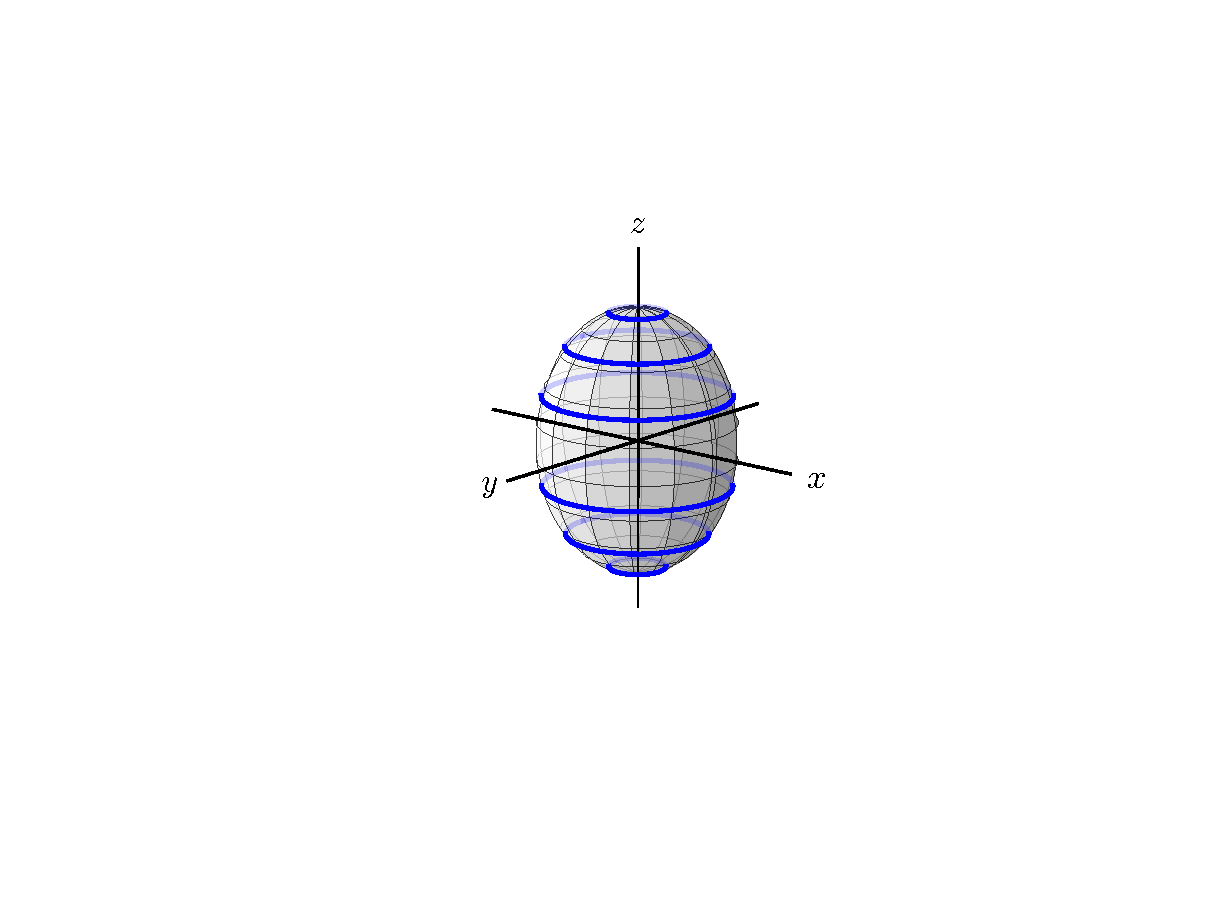
\includegraphics[trim = 50mm 50mm 50mm 20mm, clip=true ,scale=0.8]{Ellipsoid_Sphere_Biaxial}
\caption{Intersection of the sphere and ellipsoid defined in Eqn.~\eqref{eqn:
conservation of momentum biaxial} and Eqn.~\eqref{eqn: conservation of energy
biaxial} respectively for three different values of $M$ at
fixed $E$. The sphere's of radius $M$ are not visible, only the blue line shows
where they would intersect the fixed ellipsoid.}
\label{fig: plot sphere ellipse biaxial}
\end{figure}

Over times much shorter than the spin-down timescale, the energy and momentum
of our biaxial star acted on by the spin-down torque are fixed. As we have seen
above, in order to satisfy the conservation equations this means that the
angular momentum vector $J_i$ has a class of possible solution consisting of a
ring about the momentum-space $\z$.  Since $J_{i}=I_{ij}\omega^{j}$ and the
moment of inertia tensor is static, solutions for the spin-vector $\omega^j$
must also exist as points on a related circle. This related circle is exactly
the precession of $\spin$ about the $\z$ axis.

Both the energy and the momentum decay exponentially in time
due to the spin-down. As a result both the sphere and ellipsoid will shrink, but
not necessarily at the same rate. If we imagine observing the ellipsoid such
that it appears to be fixed, we may see the sphere either shrink or grow with
respect to the ellipsoid. We can parameterise the relative rate of shrinking by
considering the quantity
\begin{equation}
A(t)  = \frac{J^{2}} {2EI_{0}}.
\label{eqn: A}
\end{equation}
We could have chosen any one of the ellipsoid's semi-axes since they are all
proportional up to factors of $\epsilon_{I}$. The evolution of the spin
vector is related to the rate of change of $A$.
This quantity determines whether the sphere shrinks or grows with respect to
the ellipsoid. It is worth taking a moment to understand the different cases
which are parameterised by the sign of $\dot{A}$:
\begin{enumerate}
\item $\dot{A}>0$ The sphere grows with respect to the ellipsoid. In this case,
    the intersection circles will `close up' around the $\z$ axis. This
    agrees with the solution for $\chi=30^{\circ}$ given in
    figure~\ref{fig: NS A_NA comparison}(a). The angle between
    $\boldsymbol{\omega}$ and the $\z$ axis tends to zero while $\phi$
    monotonically increases. This describes the spin-vectors following a circle
    about the $\z$ axis, which gradually decreases in radius.
\item $\dot{A}<0$ The sphere shrinks with respect to the ellipsoid. In this
    case the intersection circles will increase in radius until $J\rightarrow
    \sqrt{2EI_{0}}$. This describes exactly the solution in
    figure~\ref{fig: NS A_NA comparison}(b): that is $a\rightarrow
    90^{\circ}$ while $\phi$ monotonically increases.
\end{enumerate}•

The sign of $\dot{A}$ tells us about the long-term evolution of the system. To
determine it, we begin by differentiating Eqn.~\eqref{eqn: A}
\begin{equation}
\dot{A}=\frac{1}{(2EI_{0})^{2}}
        \left(\frac{d}{dt}(J^{2})2EI_{0}-\frac{d}{dt}(2EI_{0})J^{2}\right),
\end{equation}
simplifying and writing in index notation such that $J^{2}=J^iJ_i$, we have that
\begin{equation}
\dot{A}=\frac{1}{E^{2}}\left(2J^{i}\dot{J}_{i}E-\dot{E}J^{i}J_{i}\right).
\end{equation}
Now the energy is purely kinetic such that
$E=\frac{1}{2}I_{ij}\omega^{i}\omega^{j}$, and therefore $\dot{E}=T^{i}\omega_{i}$.
Then, noting that $\dot{J}^{i}=T^{i}$, we have
\begin{equation}
\dot{A}=\frac{1}{E^{2}}\left(J^{i}T_{i}I_{jk}\omega^{j}\omega^{k}
                             -T^{i}\omega_{i}J^{j}J_{j}\right).
\end{equation}
For a diagonalised matrix, $I_{ij}$ has only 3 non zero components and therefore
$I_{jk}\omega^{j}\omega^{k}=(I\omega)_{j}\omega^{j}$. In addition, we can write
$J^{i}=(I\omega)^{i}$ and so we find
\begin{equation}
\dot{A}=\frac{1}{E^{2}}T^{i}\left((I\omega)_{i}\omega_{j}
        -\omega_{i}(I\omega)_{j}\right)(I\omega)^{j},
\end{equation}
finally simplifying to
\begin{equation}
\dot{A}=\frac{1}{E^{2}}T^{i}\omega_{i}\omega_{j}
        (I\omega)^{j}\left(I^{i}_{\;i}-I^{j}_{\;j}\right).
\end{equation}
Expanding the
summation on the right hand side, all terms for which $i=j$ will be zero. Working with a biaxial mass
distribution where $I_{1}=I_{2}$, then the only non-zero terms are given by 
\begin{eqnarray*}
T^{i}\omega_{i}\omega_{j}(I\omega)^{j}\left(I^{i}_{\;i}-I^{j}_{\;j}\right)&=&
T_{1}\omega_{1}I_{0}(1-\epsilon_{i})\omega^{2}_{3}
(I_{0}-I_{0}(1+\epsilon_{I}))+
T_{2}\omega_{2}I_{0}(1-\epsilon_{i})\omega^{2}_{3}(I_{0}-I_{0}(1+\epsilon_{I})) 
\\ && + 
T_{3}\omega_{3}(I_{0}(1+\epsilon_{I})-I_{0})
               (I_{0}\omega_{1}^{2}+I_{0}\omega_{2}^{2}), \\
&=& I_{0}^{2}\epsilon_{I}\omega_{3}\left(T_{3}(\omega_{1}^{2}+\omega_{2}^{2}) 
    - \omega_{3}(1+\epsilon_{I})(T_{1}\omega_{1}+T_{2}\omega_{2})\right).
\end{eqnarray*}
Working up to 1st order in $\epsI$ and transforming to spherical polar
coordinates, we then insert the spin-down torque and neglect the anomalous torque.
This yields
\begin{eqnarray*}
\dot{A}E^{2}&=& I_{0}^{2}\epsilon_{I}\omega^{3}
    \left(\frac{2R}{3c}\epsilon{A}\omega^{3}\right)
    \cos a \left([\sin \chi \cos \chi \sin a \cos \phi 
                 - \sin^{2}\chi \cos a]\sin^{2} a \right. \\
&& \left.- \cos a ([\sin \chi \cos \chi \sin a \cos \phi 
                   - \sin^{2}\chi \cos a]\cos \phi \sin a 
                   - \sin^{2}a \sin^{2}\phi)\right).
\end{eqnarray*}

Now we work in the limit $\tau_P \ll \tau_S$ where $\phi$ varies on the 
precession timescale, which is much faster than the evolution in either $a$ or $\omega$.
Therefore, we can average over a free nutation period and drop the constant
coefficients:
\begin{eqnarray*}
\langle\dot{A}\rangle &\propto& \cos a \left(-\sin^{2}a\cos a \sin^{2}\chi + 
       \frac{1}{2}\left(\sin^{2}a\cos a \cos^{2}\chi + 
       \sin^{2}a \cos a \right) \right) \\
& \propto& \cos^{2} a \sin^{2}a\left(1-\frac{3}{2}\sin^{2}\chi\right).
\end{eqnarray*}
Finally, putting all the coefficients back in, we have an expression for the averaged
rate of change of $A$ under the same assumptions made by \citet{Goldreich1970}
\begin{equation}
\langle \dot{A} \rangle =\frac{1}{\langle E\rangle ^{2}}I_{0}^{2}
                         \epsilon_{I}\omega^{6}\frac{2R}{3c}\epsilon{A} 
                         \cos^{2} a \sin^{2}a
                         \left(1-\frac{3}{2}\sin^{2}\chi\right). 
\end{equation}

This result demonstrates that only two factors determine the sign of
$\langle\dot{A}\rangle$: the sign of $\epsilon_{I}$ and the term
$1-\frac{3}{2}\sin^{2}\chi$, from which we find the critical value
$\chi_{cr}\approx55^\circ$.  The first we should expect on geometric grounds, a
change in sign of the deformation changes the geometry of the ellipsoid. The
second is in perfect agreement with the findings of \citet{Goldreich1970}.
Moreover, by calculating the condition in this way, we have found that the
critical value corresponds to a tipping point between the rates of change of
energy and angular momentum.

\FloatBarrier
\subsection{NS B in region \texorpdfstring{$\tau_{S}\sim \tau_{P}$}{}}
\label{sec: B_NA}
Unlike the previous examples, there is no comparison in the literature which
considers $\tau_{P}\sim\tau_{S}$ while neglecting the anomalous torque. This is
primarily because the similarity of the timescales means simplifying
assumptions cannot be made. The results have not been included here as they are
exactly alike with the results of NS A, except the similarity of time
scales means both the precession and alignment of the spin-vector occur on the
same timescale.

\FloatBarrier
\subsection{NS C in region \texorpdfstring{$\tau_{S}\ll \tau_{P}$}{}}
\label{sec: C_NA}
In NS C, the timescales take the ordering $\tau_{P}\gg \tau_{S}$. The limit of
this region is the spherical star
($\epsilon_{I}\rightarrow0$) discussed in section~\ref{sec: spherical}; as such
we should expect the results to be similar. Solving
the equations of motion for NS C, the spherical components of the spin axis
are given in figure~\ref{fig: NS C_NA}. Both choices of $\chi$ yield a
similar result; the polar angle $a$ tends to $\chi$ on the spin-down timescale
as anticipated by the likeness to the spherical star. In contrast, the azimuthal
angle $\phi$ appears to begin increasing monotonically before decreasing to a
constant value. It is thought that this is due to the small but non-vanishing
magnitude of $\epsilon_{I}$. In the perfectly spherical limit, we observe no
such increase in $\phi$. Therefore the small
deformation offsets the steady state solution of the spin axis from the
magnetic dipole.

For an intuitive understanding consider that the torque acts to align the spin
axis with the magnetic dipole; when this occurs the torque vanishes. Since the
mass is not spherical, non-precessing solutions exist when the spin-vector
aligns with the principal axes of the moment of inertia tensor $\x,\y$ and
$\z$. So when both effects act, the steady state solution is an intermediary
point between the two, weighted by the relative strength of each effect. In this
case, the torque dominates and so the spin-vector lies close to, but not exactly
aligned with, the magnetic dipole. During this time, the star spins down but
upon alignment the spin frequency asymptotically approaches a constant non-zero
value.
%We also plot in figure~\ref{fig: NS C_NA alpha} the angle between the spin axis and magnetic dipole $\alpha$ for NS C confirming the previous findings.
\begin{figure}[ht]
\centering
\begin{tabular}{cc}
    \subfloat[$\chi=30^{\circ}<\chi_{cr}$]{\includegraphics[width=0.495\textwidth]{{Spherical_Plot_no_anom_chi_30.0_epsI_1.0e-15_epsA_5.0e-11_omega0_1.0e4_t1_1e8}.png}}&
    \subfloat[$\chi=75^{\circ}>\chi_{cr}$]{\includegraphics[width=0.495\textwidth]{{Spherical_Plot_no_anom_chi_75.0_epsI_1.0e-15_epsA_5.0e-11_omega0_1.0e4_t1_1e8}.png}}
\end{tabular}
\caption{Plot of the spherical components of $\boldsymbol{\omega}$ for NS C. }
\label{fig: NS C_NA}
\end{figure}•

\FloatBarrier

\section{Biaxial NS including the anomalous torque}
In the previous section we considered solutions to equation \eqref{eqn: eom}
under the action of the torque in Eqn.~\eqref{eqn: torque} without the
anomalous contribution. In this section, we will include this contribution and
understand the effect it has on the character of solutions. However, before
doing so, we will first consider the appropriate reference frame in which to
view the system.

\subsection{The effective body frame}
\label{sec: effective body frame}
Working with a biaxial body and the Deutsch torque, \cite{Melatos2000}
discovered non-trivial solutions where the spin axis aligns with an unknown
angle between the magnetic dipole and the principal axis of the MOI.  This was
interpreted by Melatos as evidence for persistent precession. We show in
section \ref{sec: B} that in fact the spin-vector is aligning with another
rotating reference frame that is held at a fixed angle to the original rotating
reference frame. This reference frame, which we will call the \emph{effective} body
frame, is a direct result of the anomalous torque contribution in
Eqn.~\eqref{eqn: torque}; we will now show how this comes about from a
rearrangment of the equations of motion as first noted by \citet{Glampedakis2010}.

Writing Eqn.~\eqref{eqn: eom} with the Deutsch torque, we then manipulate it as
such
\begin{eqnarray*}
J^{i}_{\;,t}+\epsilon^{ijk}\omega_{j}J_{k} & =
& N^{i}_{\textrm{spin-down}}+
\epsA I_{0}\omega^{a}\hat{m}_{a}\epsilon^{ijk}\omega_{j}\hat{m}_{k}, \\
J^{i}_{\;,t}+
\epsilon^{ijk}\omega_{j}\left(J_{k}-\epsA I_{0}\omega^{a}\hat{m}_{a}\hat{m}_{k}\right)
& = & N^{i}_{\textrm{spin-down}}, \\
J^{i}_{\;,t}+
\epsilon^{ijk}\omega_{j}\left(I_{ka}-\epsA I_{0}\hat{m}_{a}\hat{m}_{k}\right)\omega^{a}
& = & N^{i}_{\textrm{spin-down}}.
\end{eqnarray*}
By arranging the equation this way and making use of $J_{i}=I_{ij}\omega^{j}$,
we can write an effective moment of inertia tensor given by
\begin{align}
\begin{split}
I'_{jk}&=I_{jk}-I_{0}\epsA\hat{m}_{j}\hat{m}_{k}, \\
&= \left[
\begin{array}{ccc}
I_{0}(1-\epsA\sin^{2}\chi) & 0 & -I_{0}\epsA\sin\chi \cos \chi \\
0 & I_{0} & 0 \\  -I_{0}\epsA\sin\chi \cos \chi& 0 &
I_{0}(1+\epsilon_{I}-\epsA\cos^{2}\chi)
\end{array}
\right].
\end{split}
\label{eqn: effective MOI}
\end{align}
Note that we will use the prime to denote the effective body frame axis.

We can calculate the eigenvalues of the effective MOI, which are given by
\begin{align}
\lambda_{2}=I_{0}, &&&
\lambda_{\pm}=\frac{I_{0}}{2}
\left(2+\epsilon_{I}-\epsA\pm
\sqrt{\epsA^{2}+\epsilon_{I}^{2}-2\epsA\epsilon_{I}\cos(2\chi)}\right).
\end{align}
If we diagonalise this effective moment of inertia tensor, these eigenvalues
are the diagonal entries, and the associated eigenvectors are the principal
axes of the effective body frame. The eigenvalues always take the ordering
\begin{equation}
\lambda_{+}>I_{0}>\lambda_{-}.
\end{equation}•
Defining the effective body frame axis by $\boldsymbol{e_{i}}$, it is natural to
associate $\boldsymbol{e}_{2}$ with the
$\boldsymbol{\hat{y}}$ of the body frame axis such that they are always
parallel. Since the other axes must be orthonormal, the transformation must
consist of a rotation in the $x-z$ plane by an angle $\beta$. We are
free to set the $\boldsymbol{e}_{3}$ axis to always take the largest eigenvalue
and then define $\beta$ as the angle made by $\3$ with the
$\hat{\boldsymbol{z}}$ axis. $\beta$ is then given by
\begin{equation}
\beta = \arctan\left(\frac{\boldsymbol{e}_{3,1}}{\boldsymbol{e}_{3,3}}\right)
=\arctan\left( \frac{ \epsilon_{I}-\epsA\cos(2\chi)-
              \sqrt{\epsA^{2}+\epsilon_{I}^{2}-2\epsA\epsilon_{I}\cos(2\chi)}}
              {2\epsA\sin\chi \cos\chi}\right).
\label{eqn: beta}
\end{equation}•
A schematic of the various angles and axes is given in
figure~\ref{fig: schematic}
\begin{figure}[ht]
\centering
 	\begin{tikzpicture}[scale=1.75] 

	% Define some things

	\def\costhirty{0.8660256}
	\def \mag{1.5}

	\def\cosbeta{0.984}
	\def\sinbeta{0.173}

	% Colors
	\colorlet{anglecolor}{blue!80!black}
	\colorlet{sincolor}{red}
	\colorlet{tancolor}{orange!80!black}
	\colorlet{coscolor}{blue}

	% Styles
	\tikzstyle{axes}=[]
	\tikzstyle{important line}=[very thick]
	\tikzstyle{information text}=[rounded corners,fill=red!10,inner sep=1ex]

	% Draw the shaded star
	\def\R{1.0} % sphere radius
	\filldraw[ball color=white] (0,0) ellipse (1.05 and 1.0);

	% Draw the angles
	\draw[draw=red!80!black] (0,0) -- (0pt,7mm) arc(90:30:7mm);
	  \draw (45:6mm) node[red!80!black] {$\chi$};


	\draw[draw=blue!80!black] (0,0) -- (0pt,6mm) arc(90:60:6mm);
	  \draw (75:5mm) node[blue!80!black] {$a$};

	\draw[draw=magenta] (0,0) -- (-8.1*\sinbeta mm, 8.1*\cosbeta mm) arc(100:60:8.1mm);
	  \draw (80:9.2mm) node[magenta] {$a'$};

	%\draw[draw=green!60!black] (0,0) -- (12mm*\costhirty,12mm*0.5) arc(30:60:12mm);
	 % \draw (45:11mm) node[green!60!black] {$\alpha$};



	% Draw the body frame axis
	\draw[->] (-1.5,0) -- (1.5,0) node[right] {$\x$};
	\draw[->] (0,-1.5) -- (0,1.5) node[above] {$\z$};

	% Draw the effective body frame axis
	\draw[draw=green!60!black] (0,0) -- (0,13mm) arc(90:100:13mm);
	  \draw (95:11mm) node[green!60!black] {$\beta$};

	\draw[green!60!black, dashed,->] (-1.5*\cosbeta,-1.5*\sinbeta) -- (1.5*\cosbeta,1.5*\sinbeta) node[green!60!black,right] {$\1$};
	\draw[green!60!black, dashed,->] (1.5*\sinbeta,-1.5*\cosbeta) -- (-1.5*\sinbeta,1.5*\cosbeta) node[green!60!black,above] {$\3$};




	% Define omega to have unit magnitude and lie at 30 degrees to the z axis
	{\draw[color=blue!80!black,very thick,->] (0,0,0) -- (\mag*0.5,\mag*\costhirty) node[anchor=south]{$\Omega$};}%

	% Define m to have unit magnitude and lie at 60 degrees to the z axis
	{\draw[color=red!80!black,very thick,->] (0,0,0) --(\mag*\costhirty,\mag*0.5) node[anchor=south]{$\hat{m}$};}%

	\end{tikzpicture}

\caption{Schematic of the two sets of axes for an arbitrary $\beta$. Note that
$\beta$ is defined to be positive for a right hand rotation about the $\y$ axis
which is defined to be into the page.}
\label{fig: schematic}
\end{figure}•

\paragraph{Understanding the effective body frame}
The effective body frame is a simple rotation of the axis defined by the moment
of inertia tensor to accommodate the effects of the anomalous torque. We work
in a case where the rotation is in only the $x-z$ plane by an angle
$\beta$.

To understand when this becomes significant we plot $\beta$ as a function of
$|\epsA/\epsilon_{I}|$ in figure~\ref{fig: beta}. When $|\epsA \ll
\epsilon_{I}|$, such that the anomalous torque effects are negligible, we
recover the usual moment of inertia tensor. That is, $\beta=0$ or
$\beta=\pi/2$, dependent on the sign of $\epsilon_{I}$. This is a consequence
of choosing $\3$ to take the largest eigenvalue.  In the opposing limit
$|\epsA \gg \epsilon_{I}|$, in which the magnetic deformation dominates,
the sign of the elastic deformation no longer splits the solutions and in both
cases $a$ tends to $\chi - 90^{\circ}$. This means the effective body frame always
aligns the $\1$ axis (which has the smallest eigenvalue) with the magnetic
dipole.
\begin{figure}[ht]
\centering
\includegraphics[scale=0.4]{{beta}.png}
\caption{Plot of $\beta$ as a function of the ratio
    $|\epsA/\epsilon_{I}|$ for a prolate, $\epsilon_{I}<0$, and oblate,
    $\epsilon_{I}>0$, mass distribution.  In the limit $\epsA \gg
    \epsilon_{I}$ for both the oblate and prolate cases, the effective body
    frame aligns with the magnetic dipole. In the opposing limit the magnetic
    dipole has little effect and the effective body frame aligns with the
    principal axis of the moment of inertia. There is a smooth transition
    between these two extremes when $\epsA \sim \epsilon_{I}$. The
    splitting into oblate and prolate solutions results from choosing to
    associate $\boldsymbol{e}_{3}$ with the largest eigenvalue.}
\label{fig: beta}
\end{figure}

We will show in the following that, when the anomalous torque is included, it
is the effective body frame to which the system aligns on the spin-down
timescale (much as it is the body frame to which the system aligns when the
anomalous torque contribution was neglected in Sec.~\ref{sec: biaxial NS
with no anomalous torque}).

For the three NSs (A, B, and C) representative of different orderings of the timescales, all
three have a non-zero $\beta$. To familiarise the reader with the magnitudes in
the different regions, in Table~\ref{tab: A B C params} we list the relevant
timescales and $\beta$ for each of the three NSs.
\begin{table}[ht]
{\footnotesize
\centering
	\begin{tabular}[ht]{|c|c|c|c|c|c|c|c|c|}\hline
NS &  $\epsilon_{I}$  & $\epsA $ & 	$B_{S} \; $[Gauss] & $\tau_{S}$ [s] & $\tau_{A}$ [s] & $ \tau_{P}$  [s] & $\beta (\chi=30^{\circ})$ & $\beta(\chi=75^{\circ})$ \\ \hline
A & $  1.0\times 10^{-9}  $ & $  5\times 10^{-9}  $ & $  1.3\times 10^{13}  $ & $  3.6\times 10^{8}  $ & $  1.3\times 10^{7}  $ & $  6.3\times 10^{5}  $ & $ -1.27^{\circ} $& $ -0.7^{\circ} $ \\
B & $  0.4\times 10^{-10}  $ & $  5\times 10^{-9}  $ & $  1.3\times 10^{13}  $ & $  3.6\times 10^{8}  $ & $  1.3\times 10^{7}  $ & $  1.6\times 10^{7}  $ & $ -35.447^{\circ} $& $ -8.35^{\circ} $ \\
C & $  1.0\times 10^{-15}  $ & $  5\times 10^{-9}  $ & $  1.3\times 10^{13}  $ & $  3.6\times 10^{8}  $ & $  1.3\times 10^{7}  $ & $  6.3\times 10^{11}  $ & $ -60.0^{\circ} $& $ -15.0^{\circ} $ \\ \hline
	\end{tabular}•}
\caption{Table of relevant values for the selected points. }
\label{tab: A B C params beta}
\end{table}

In the following, we will present results in the effective body frame axis. These
are calculated by numerical evolution of the Euler rigid-body equations with the full
torque Eqn.~\eqref{eqn: torque}. Then, in the post-processing stage, we apply the
effective body frame transformation (a rotation by the angle $\beta$).

\subsubsection{Phase space}

The introduction of the anomalous torque means we must also consider the
anomalous torque timescale as given in equation \eqref{eqn: torque timescales}. Three
timescales can take six orderings. However, the spin-down and anomalous timescale
obey the following relation
\begin{equation}
\tau_{S} = \frac{3c}{2R}\frac{1}{\nu_{0}}\tau_{A}.
\end{equation}
The coefficient $2R/3c$ effectively measures the importance of special
relativity at the surface of the star. Since we expect $c\gg R \omega_{0}$, this
means that only three physical orderings exist:
\begin{enumerate}
\item Region A: $\tau_{S}>\tau_{A}> \tau_{P}$
\item Region B: $\tau_{S}>\tau_{P}> \tau_{A}$
\item Region C: $\tau_{P}>\tau_{S}> \tau_{A}$
\end{enumerate}•

We can therefore update the phase space of possible solutions with the
additional anomalous timescale; the result is given in figure~\ref{fig: phase
space}.

\begin{figure}[ht]
\centering
\includegraphics[scale=0.5]{{phase_space}.png}
\caption{Phase space diagram including the anomalous torque contributions.}
\label{fig: phase space}
\end{figure}•

\FloatBarrier
\subsubsection{NS A in region \texorpdfstring{$\tau_{S}>\tau_{A}>\tau_{P}$}{}}
\label{sec: A}

We expect the alignment of the spin axis to agree with the findings in section
\ref{sec: A_NA} and study the changes in behaviour due to the introduction of
the anomalous torque. Working in the effective body frame axis rotates the
solutions by a few degrees as shown in Table~\ref{tab: A B C params beta}.
Plotted in figure~\ref{fig: NS A} are the spherical components of the spin
vector in the effective body frame axis. This can be compared with the result
in figure~\ref{fig: NS A_NA}, which is the same system without the anomalous
torque.

\begin{figure}
\centering
\begin{tabular}{cc}
    \subfloat[$\chi=30^{\circ}<\chi_{cr}$]{\includegraphics[width=0.495\textwidth]{{Spherical_Plot_Transform_chi_30.0_epsI_1.0e-9_epsA_5.0e-11_omega0_1.0e4_eta_1.0e-4}.png}} &
    \subfloat[$\chi=70^{\circ}>\chi_{cr}$]{\includegraphics[width=0.495\textwidth]{{Spherical_Plot_Transform_chi_75.0_epsI_1.0e-9_epsA_5.0e-11_omega0_1.0e4_eta_1.0e-4}.png}}
\end{tabular}
\caption{Plot of the spherical components of the spin-vector during the spin-down of NS A.}
\label{fig: NS A}
\end{figure}•

The final state alignment agrees well with results neglecting the anomalous
torque for both values of $\chi$. For $\chi = 30^{\circ}$, the intermediate
behaviour appears similar to those shown in section~\ref{sec: A_NA}. For
$\chi=75^{\circ}$, we have a large discontinuity in the
solution suggesting a significant difference between solutions when including
the anomalous torque. To understand the cause of this, we return to the
geometric argument made in Sec.~\ref{sec: A_NA}.

\paragraph{A geometric interpretation}
Working in the effective body frame for which the effective moment of inertia
tensor is triaxial, the conservation of energy equation is
\begin{equation}
1 = \frac{J_{1}^{2}}{2\lambda_{-}E}+\frac{J_{2}^{2}}{2I_{0}E}+\frac{J_{3}^{2}}{2\lambda_{+}E},
\label{eqn: conservation of energy triaxial}
\end{equation}
while the conservation of momentum remains as in Eqn.~\eqref{eqn: conservation of momentum biaxial}, that is
\begin{equation}
J^{2}  =  J_{1}^{2}+J_{2}^{2}+J_{3}^{2}.
\label{eqn: conservation of mass triaxial}
\end{equation}

In analogue to the geometric argument of  Sec.~\ref{sec: A_NA}, the first equation,
the conservation of momentum, describes a triaxial ellipsoid with semi axes
given by $\sqrt{2\lambda_{-}E}$, $\sqrt{2I_{0}E}$, and $\sqrt{2\lambda_{+}E}$, while
the conservation of energy still describes a sphere of radius $J$. In order to
satisfy both conservation equations, the sphere and ellipsoid must intersect
bounding the radius of the sphere by
\begin{equation}
2E\lambda_{-}<J^{2}<2E\lambda_{+}.
\end{equation}

In the case of a biaxial moment of inertia, we found that solution for which both
conservation laws are satisfied, corresponded to circles around the $\z$ axis.
Now that we have a triaxial MOI (due to the addition of the anomalous torque),
the solutions correspond to the intersection of the triaxial ellipsoid with the
sphere, for which there are three distinct types of
intersections as drawn in figure~\ref{fig: sphere ellipsoid}.
\begin{figure}[ht]
\centering
\begin{tabular}{ccc}
    \subfloat[$2E\lambda_{-}<J^{2}<2EI_{0}$]
             {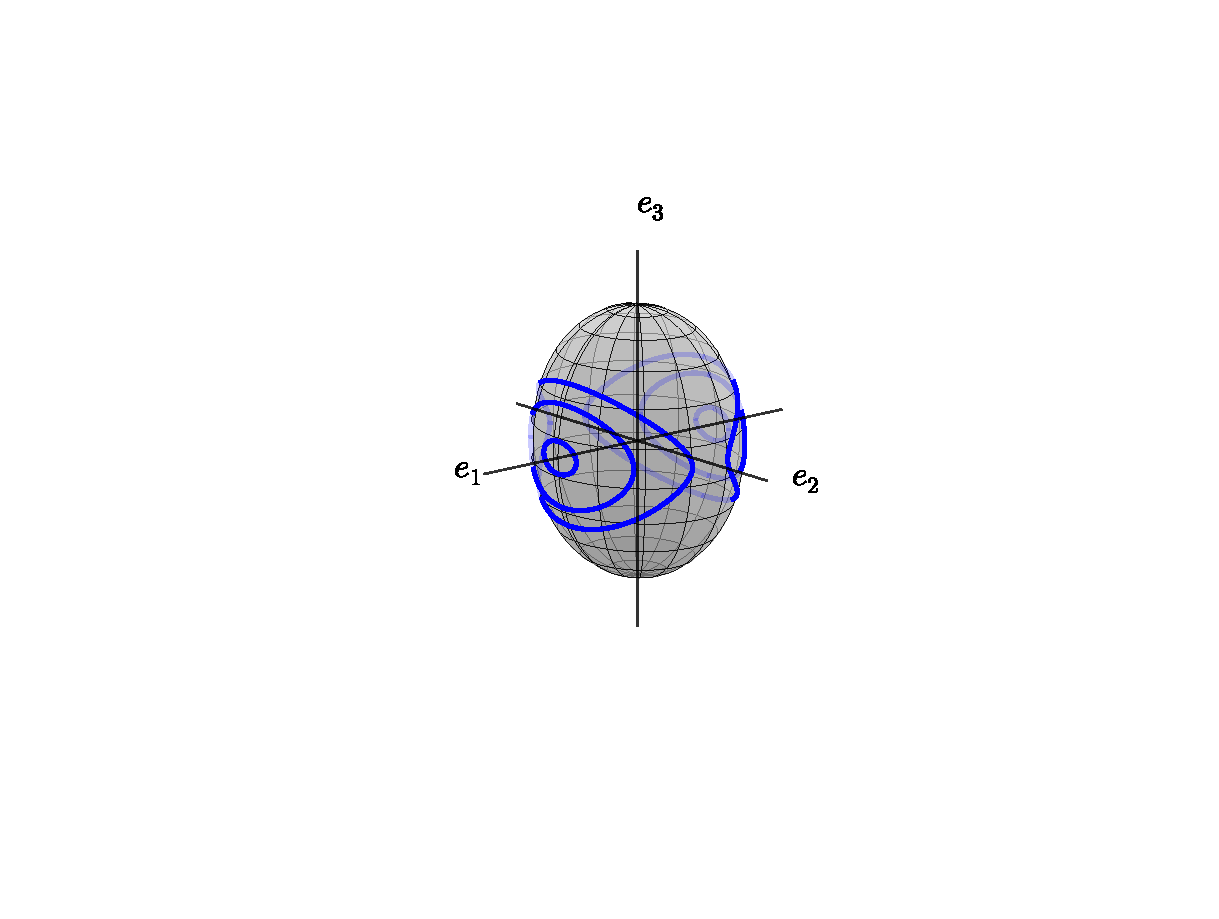
\includegraphics[trim = 70mm 50mm 50mm 20mm, clip=true, width=0.333\textwidth]
             {Ellipsoid_Sphere_low.pdf}} &
    \subfloat[$ J^{2} = 2EI_{0}$]
             {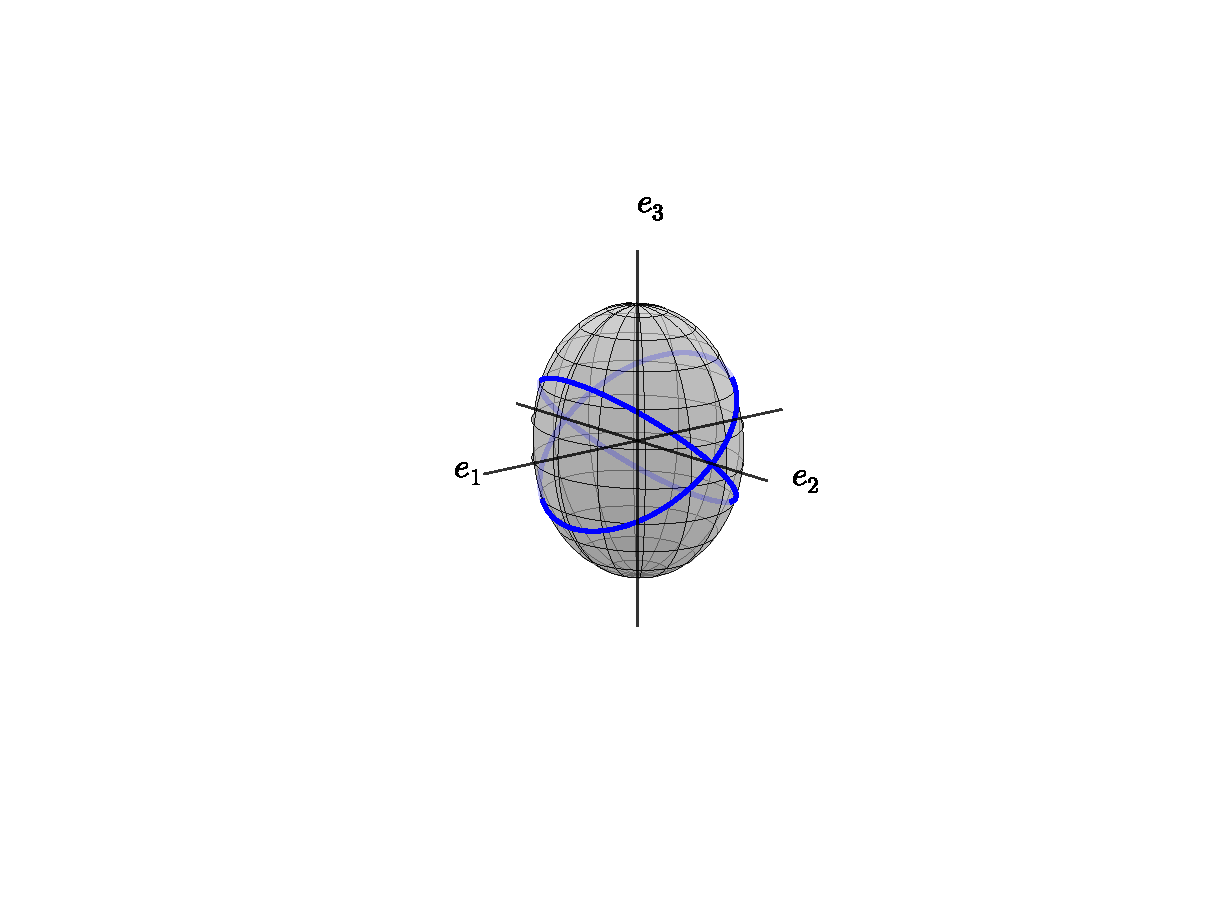
\includegraphics[trim = 70mm 50mm 50mm 20mm, clip=true, width=0.333\textwidth]
             {Ellipsoid_Sphere.pdf}} &
    \subfloat[$2EI_{2}<J^{2}<2EI_{3}$]
             {\includegraphics[trim=70mm 50mm 50mm 20mm, clip=true ,width=0.333\textwidth]
             {{Ellipsoid_Sphere_high}.pdf}}
\end{tabular}
\caption{Intersection of the sphere and ellipsoid defined in Eqn.~\eqref{eqn:
conservation of energy triaxial} and Eqn.~\eqref{eqn: conservation of mass
triaxial} respectively for three different values of $M$ at
fixed $E$}
\label{fig: sphere ellipsoid}
\end{figure}

Each of these types of intersection can be understood through the orderings of
the radius of the sphere and the sizes of the three semi-axes of the ellipsoid:
\begin{enumerate}[(a)]
\item $2E\lambda_{-}<J^{2}<2EI_{0}$. In this region, curves form two sets of
    complete loops around the $\1$ axis. As $J^{2} \rightarrow 2E\lambda_{-}$
    the intersection loops will close up about the $\1$ axis.
\item $J^{2} = 2EI_{0}$. This is a special case in which the intersection forms two
    closed ellipses
\item $2EI_{0}>J^{2}>2E\lambda_{+}$. In this region, curves form two sets of
    complete loops around the $\3$ axis. As $J^{2} \rightarrow 2E\lambda_{+}$
    the intersection loops will close up about the $\3$ axis.
\end{enumerate}

Now that we have understood the possible types of solution via the intersections
of the sphere and ellipsoid, we can understand the cause of the unusual behaviour
in Fig.~\eqref{fig: NS A}(b). First, we note that
all simulations begin in the same initial state. As previously observed,
changing $\chi$ through the critical value changes the sign of $\dot{A}$ and
hence whether the sphere will grow or shrink with respect to the ellipsoid. So
for $\chi=30^{\circ}$, the sphere grows with respect to the ellipsoid
($\dot{A}>0$) ending up with the loops closing up about the $\3$ axis. For
$\chi=75^{\circ}$ the sphere shrinks with respect to the ellipsoid
($\dot{A}<0$) ending up with the loops closing up about the $\1$ axis. The two
end states are then the (a) and (c) pictures in figure \ref{fig: sphere ellipsoid}.

If they both begin from the same initial configuration, then one of them must pass through
the special $J^{2}=2EI_{0}$ state corresponding to figure \ref{fig: sphere ellipsoid}(b).
When this happens, we will observe a change in the axis about which the solution
precesses.

Both sets of solution start with the solution precessing about the $\3$ axis
($\phi$ monotonically increasing) corresponding to figure \ref{fig: sphere ellipsoid}(c).
In figure~\ref{fig: NS A}(b), the discontinuity is in fact exactly the point
when the solution changes the axis of precession.

To better understand this, we plot the data from the
$\chi=75^{\circ}$ simulation (\ref{fig: NS A}(b)) in figure~\ref{fig: NS A 3D}. Firstly in (a),
we project the spherical components onto the unit sphere and choose three
short sections of data. This shows that at early times (in blue) the solution
precesses about the $\3$ axis. During the discontinuity (in red) the solution
shows similarities with the $J^{2}=2EI_{0}$ case from figure~\ref{fig: sphere
ellipsoid}. Finally at late times, in black, the solution precesses about
the~$\1$~axis. In figure~\ref{fig: NS A 3D}(b) we also plot the solution in
3D during the apparent discontinuity. This again shows that the solution goes
through a change of the axis about which it precesses.

\begin{figure}
\centering
\begin{tabular}{cc}
    \subfloat[]{\includegraphics[trim = 30mm 30mm 30mm 30mm, clip=true , width=0.495\textwidth]{{Angle_Space_Plot_3D_chi_75.0_epsI_1.0e-9_epsA_5.0e-11_omega0_1.0e4_eta_1.0e-4}.png}} &
    \subfloat[]{\includegraphics[trim = 30mm 30mm 30mm 30mm, clip=true , width=0.495\textwidth]{{ThreeD_Plot_Cartesian_chi_75.0_epsI_1.0e-9_epsA_5.0e-11_omega0_1.0e4_eta_1.0e-4}.png}}
\end{tabular}
\caption{Numerical solutions for NS A plotted on the unit sphere in the
body frame axis. Figure (a) shows three distinct time steps; blue, the time before the
discontinuity, red is during the discontinuity, and black is some time after.
Figure (b) demonstrates the solution during the discontinuity, the changing colour is
used to illustrate the evolution with time, progressing from green to blue.}
\label{fig: NS A 3D}
\end{figure}•

\FloatBarrier
\subsubsection{NS B in region \texorpdfstring{$\tau_{S}> \tau_{P}>\tau_{A}$}{}}
\label{sec: B}

This NS takes on a new significance having included the anomalous torque -
we can now make a comparison with the work of \citet{Melatos2000}. In this
work, Melatos found that when the precession timescale and anomalous torque
timescales are comparable, the solutions involve \emph{persistent precession}. Specifically,
this is defined as the polar angle $a$ tending to a constant, non-zero value with the
nutation amplitude (oscillations in $a$) either decaying or remaining constant.
Because the spin-vector has not aligned with a principal axis of the moment of
inertia, this was interpreted as the spin-vector undergoing persistent
precession. Working in the body frame axis, we confirm that $a\ne\pi/2$ at the
end of the evolution in figure~\ref{fig: NS B}(a).

Transforming to the effective body frame in figure~\ref{fig: NS B}(b), we
find that the spin-vector in fact aligns with the principal axis of the
effective moment of inertia ($a \rightarrow \pi /2$).  Therefore, the persistent
precession angle found by Melatos is precisely the angle $\beta$.
The spin-vector has therefore aligned with the principal axis of
the effective moment of inertia tensor associated with the smallest eigenvalue.
Since the azimuthal angle is constant, we argue that this is not persistent
precession: the moment spin-vector aligns with the effective body frame at which
point the precession ceases.

\begin{figure}[ht]
\centering
\begin{tabular}{cc}
    \subfloat[In the body frame axis]
             {\includegraphics[width=0.495\textwidth]
             {{Spherical_Plot_chi_75.0_epsI_4.0e-11_epsA_5.0e-11_omega0_1.0e4_t1_2.0e8}.png}} &
    \subfloat[In the effective body frame axis]
             {\includegraphics[width=0.495\textwidth]
             {{Spherical_Plot_Transform_chi_75.0_epsI_4.0e-11_epsA_5.0e-11_omega0_1.0e4_t1_2.0e8}.png}}
\end{tabular}
\caption{Plot of the spherical components of $\boldsymbol{\omega}$ for NS B}
\label{fig: NS B}
\end{figure}•

\FloatBarrier

\subsubsection{NS C in region \texorpdfstring{$\tau_{P}> \tau_{S}>\tau_{A}$}{}}
\label{sec: C}

In figure \ref{fig: NS C}, for all values of $\chi$, the spin-vector is found
to align with the effective body frame $\1$ axis.  In this limit ($\epsA \gg
\epsilon_{I}$ and so from figure~\ref{fig: beta}), we see that the $\1$ axis
aligns with the magnetic dipole. This agrees with the results for a spherical
star in which $\epsilon_{I} \rightarrow 0$. The addition of the anomalous
torque introduces oscillations on the anomalous torque timescale.

\begin{figure}[ht]
\centering
\begin{tabular}{cc}
    \subfloat[$\chi=30^{\circ}<\chi_{cr}$]{\includegraphics[width=0.495\textwidth]
             {{Spherical_Plot_Transform_chi_30.0_epsI_1.0e-15_epsA_5.0e-11_omega0_1.0e4_t1_1e8}.png}} &
    \subfloat[$\chi=75^{\circ}>\chi_{cr}$]{\includegraphics[width=0.495\textwidth]
             {{Spherical_Plot_Transform_chi_75.0_epsI_1.0e-15_epsA_5.0e-11_omega0_1.0e4_t1_1e8}.png}}
\end{tabular}
\caption{Plot of the spherical components of $\boldsymbol{\omega}$ for NS
C. }
\label{fig: NS C}
\end{figure}

\FloatBarrier

\section{Conclusion: alignment of the spin-vector}
This simple model, comprising an elastic body supporting a biaxial strain and
acted on by an electromagnetic torque, has been validated against known
analytic results. Neglecting the anomalous torque, we expand on the results of
\citet{Goldreich1970}: the dependency on $\chi$ of the spin-vector alignment is
related to the ratios of the loss of angular momentum and energy.

When using the anomalous torque we introduced the effective body frame.
In all cases we find that the spin-vector aligns with
the principal axis of this effective moment of inertia tensor. For NSs in
region A of figure~\ref{fig: phase space}, the effective moment of inertia tensor
is triaxial. This means that it is possible for the spin-vector to precess
about either of the principal axes associated with the smallest and largest
eigenvalue. As a result, solutions can admit apparent discontinuities, under
inspection these are revealed as the points where the precession changes
between the two axes.

\section{Conclusion: understanding the wobble angle}

%This wobble angle is still incomplete, because the EM torque will in fact cause
%the angular momentum vector to wobble as well: it is not fixed in space.
%The magnitude of this time varying component is give by
%\begin{equation}
%|\dot{\J}| \sim J \omega \hat{\theta}.
%\end{equation} 
%The magnitude of this can be equated to the magnitude of the spin-down torque
%given by
%\begin{equation}
%|T_{\mathrm{sd}}| = I_{0}|\dot{\spin}|,
%\end{equation}
%rearranging for the angle between the spin-vector and angular momentum yields
%\begin{equation}
%    \hat{\theta} = \frac{I_{0}\dot{\omega}}{I \omega^{2}} = \frac{P}{\tauS}.
%\end{equation}
%Finally, substituting in Eqn.~\eqref{eqn: theta hat theta} we find that the magnitude
%of variations in $\theta$ due to the wobble of the angular momentum vector are
%given by
%\begin{align}
%\theta \sim \frac{P}{\tauS}\frac{1}{\epsI} = \frac{\tauP}{\tauS}.
%\end{align}
%In the case where the precession time-scale is similar to the spin-down time
%scale this effect may be important. However, for all realistic neutron stars,
%we can only observe precession if it occurs on our observation time-scale $\sim
%40$~yrs which is much shorter than the spin-down time-scale.
%
%In conclusion the wobble angle defined in \citet{Jones2001} is incomplete. However,
%the variations due to the wobble of the angular momentum vector will not be
%important for realistic neutron stars. The variations due to the effective
%body-frame rotation could potentially be important for stars with strong
%magnetic fields, therefore we will refer to Eqn.~\eqref{eqn: wobble angle} as
%the wobble angle.

%\section{Connection with the known NS population}
%\label{sec: Connection with the known NS population}
%TBD

%\label{sec: connection with pp}
%
%Having an understanding of how the different types of solutions behave, we now
%compare this with the known NS population to estimate which types of solutions
%are physically relevant.
%
%Using a large value of the initial spin period will skew the phase diagrams in
%figure \ref{fig: phase space}. We therefore present a more realistic phase
%diagram in figure~\ref{fig: phase space for actual spin frequency} for a
%realistic spin frequency of $\nu=1.6$~Hz. The strongest candidates displaying a
%periodic signal, which may be explained by precession, were collected in
%\citet{Lyne2010}. The 18 NSs where listed along with their: spin frequency,
%frequency derivative and the peak fluctuation frequency of the power spectra
%$F$. It is a standard calculation to find the magnetic field from the first two
%parameters:
%
%\begin{equation}
%B_{s} = 3.3 \times^{19}\sqrt{-\dot{\nu}\nu^{-3}},
%\end{equation}
%see \citet{Lyne2012book} for more details. We now make the assumption that the
%fluctuations at frequency $F$ are due to free precession such that the elastic
%deformation may be calculated by rearranging equation \ref{fig: free
%precession}:
%\begin{equation}
%\epsilon_{I} = \frac{1}{\nu F}.
%\end{equation}•
%We use this as a first approximation to discuss the types of solution that may
%be relevant to the NS population, but recognise that we have yet to account
%for the damping due to any superfluid core.
%\begin{figure}[ht]
%\centering
%	\centering
%    \includegraphics[width=0.6\textwidth,trim=0mm -10mm 0mm 0mm]
%                    {{Phase_Space_Realistic_Omega0}.png}
%\caption{Phase space of the orderings of the three timescales using a realistic
%    value of the spin frequency. This can be compared with estimates of where
%    the NSs from \citet{Lyne2010} sit assuming the periodic oscillations
%are due to precession.}
%\label{fig: phase space for actual spin frequency}
%\end{figure}•
%Plotting the results in figure~\ref{fig: phase space for actual spin frequency} we observe that all NSs exist in Region A of the phase diagram.
%
%\FloatBarrier
%
%\subsection{Future work}
%Having validated that our simple framework  agrees with the results in the
%literature we can look forward to see how it may be used and what is not yet
%included. Recent work by \citet{Seymour2012} has found evidence for chaotic
%behaviour in several NSs, they predict that the governing equations should
%be 3 non linear coupled ODEs with one variable the spin-down. Our model fits
%such a system and so we aim to search for any chaotic behaviour in our results
%and use this as an observational test of out model. The primary objection to
%precession as an underlying mechanism for timing noise is that any fluid core
%of the NS will damp the precession. We aim to reproduce this result by
%adding a second core following the frictional coupling method of
%\citet{Bondi1955}. Adding random kicks during the spin-down we can  evaluate
%the suggestion of \citet{Cordes1993} that such kicks will excite the
%precession. In addition we can check the ideas of \citet{Cordes2013} that the
%periodicity results from stochastic resonance. Comparing the size and frequency
%of kicks with realistic models  will help to ascertain the validity of this
%idea.

\begin{subappendices}
\section{Considerations for the timescales}\label{sec: timescales}
We have used the ordering of the three timescales at $\omega_{0}=\omega(t=0)$
to categorise the results. However, clearly the magnitude of the spin-vector
will decrease and the different dependencies on the spin-vector could cause a
`crossing' of the timescales producing unexpected results. Writing the
timescales as 
\begin{equation}
\tau_{P}(t)=\frac{2\pi}{\epsilon_{I}\omega(t)}, \;\;\;\;\; 
\tau_{A}(t)=\frac{2\pi}{\epsilon_{A}\omega(t)},  \;\;\;\;\; 
\tau_{S}(t)=\frac{3c}{2R}\frac{2\pi}{\epsilon_{A}\omega(t)^{2}},
\end{equation}
only $\tau_{S}$ could cross with the other two timescales since the spin-down
and anomalous timescales obey $\tau_{S}>\tau_{A}$ provided that 
\begin{equation*}
\omega(t)>\frac{3c}{2R}.
\end{equation*}•
This condition is satisfied by setting the initial rotational spin frequency at
less than $\omega_{0} \sim 10^{4}$ [Hz rad], that is the star should not break
special relativity. At later times, the spin frequency will decay and so this
condition is still satisfied.

For the anomalous torque and precession timescale crossings, two cases exists:
either the deformations are such that the spin-down timescale is initially larger than
the precession timescale (region A and B) or, as in region C, the precession
timescale is larger than the spin-down timescale. Let us consider the first case:
\begin{equation}
\tau_{S}>\tau_{P} \;\;\; 
\Rightarrow \omega(t)<\frac{3c}{2R}\frac{\epsilon_{I}}{\epsilon_{A}},
\end{equation}•
in this particular state $\epsilon_{I}>\epsilon_{A}$ and so as in the previous
case while the spin-vector decays, this inequality is always satisfied and the
orderings remain the same. In the other case we have
\begin{equation}
\tau_{P}>\tau_{S} \;\;\; 
\Rightarrow \omega(t)>\frac{3c}{2R}\frac{\epsilon_{I}}{\epsilon_{A}}.
\end{equation}
In this case, it is possible for the timescales to cross at
$\omega_{cr}=\frac{3c}{2R}\frac{\epsilon_{I}}{\epsilon_{A}}$. For pulsar C this
corresponds to a rotational spin frequency of $0.9$ [Hz rad], which is four
orders of magnitude smaller than the initial frequency. For this reason, we can
rule out this crossing of the timescales as an important factor in
calculations. 



\end{subappendices}

\biblio

\end{document}
